\documentclass[conference]{IEEEtran}
\usepackage[english]{babel}
\usepackage{multicol}
\usepackage{multirow}
\usepackage{url,hyperref,graphicx,float,times}
\usepackage{textcomp}
\usepackage{cite}
\usepackage[caption=false,font=footnotesize]{subfig}
\usepackage{placeins}
%\usepackage{flafter}

\usepackage{url}
\usepackage{listings}
% \usepackage{sectsty}
% \usepackage{authblk}
% \graphicspath{{../pdf/}{../jpeg/}}
% \DeclareGraphicsExtensions{.pdf,.jpeg,.png}

\author{
\IEEEauthorblockN{
\bf
Sheng-Wen Cheng\IEEEauthorrefmark{1},
Shao-Hua Wang\IEEEauthorrefmark{2},
Po-Sheng Chen\IEEEauthorrefmark{2},
Keng-Fu Hsu\IEEEauthorrefmark{2},
Chun-Yi He\IEEEauthorrefmark{2},
Ching-Chun (Jim) Huang\IEEEauthorrefmark{3}}

\IEEEauthorblockA{
\IEEEauthorrefmark{1}Department of Computer Science and Information Engineering, Providence University, Taiwan}

\IEEEauthorblockA{
\IEEEauthorrefmark{2}Department of Engineering Science, National Cheng Kung University, Taiwan}
    
\IEEEauthorblockA{
\IEEEauthorrefmark{3}Department of Computer Science and Information Engineering, National Cheng Kung University, Taiwan}
}


\begin{document}

\title{Puyuma: Linux-based RTOS experimental platform for constructing self-driving miniature vehicles}

\maketitle

\begin{abstract}
A holistic design and cost-efficient platform to construct self-driving systems is presented, with an emphasis on Linux-based software architectures for computer vision, control system, and inter-vehicle communication. Starting with an executable specification of autonomous car application, subsequent transformations are performed across different levels of abstraction until the final implementation is achieved. The software partitioning is facilitated through the integration of ROS and OpenCV in the same design environment, as well as closed-loop control algorithms and Linux in the run-time system. We built a rapid prototyping based on fundamentally open source technologies and hardware under 100 dollars USD, which allows developers to be explored and evaluated in realistic conditions efficiently. Using lane departure and the corresponding performance speedup, we show that our platform reduces the design time, while improving the verification efforts, with the aid of tweaked real-time executives.
\end{abstract}

\section{Introduction}
As an example of autonomous vehicles, the Google Car has already succeeded in covering thousands of miles of real-road driving \cite{autonomous} with the promising benefits by increasing traffic efficiency \cite{traffic-flow}, reducing pollution \cite{reduce-pollution}, and eliminating up to 90\% of traffic accidents \cite{traffic-accident}. However, it is not straightforward for most people to build autonomous vehicles due to very high bill of materials (BOM) and insufficient system software infrastructure, that prevents from potential innovations and collobrations, especially to arising maker movement \cite{maker}.

The goal of this research was to adapt open source foundation and to design algorithms for a self-driving miniature vehicle, which should be able to reliably follow lane markings, overtake stationary obstacles, and park automatically for inexpensive hardware configurations. We explicitly explore the possibility to not only exploit hardware components but also the software/hardware interface to read data from sensors and to control the actors for steering and acceleration, which was evaluated by various system services of the incorporation of the real-time extension for GNU/Linux. Afterwards, a short overview of the development process and the evaluation of the software is presented.

\section{Related Work}

In this section, we concentrate on currently available frameworks for the development of component-based embedded automotive and robotics software.

In 2016, MIT CSAIL took students on a trip to "Duckietown" \cite{Duckietown} to create self-driving taxis that can navigate the roads of a model city with just a single on-board camera and no pre-programmed maps. Students developed algorithms to read traffic signs and notice pedestrian-ducks, and learned to integrate different disciplines like control theory, machine learning, and computer vision into their systems. Eventually, MIT distributes all the lecture materials, middleware, drivers, ROS modules, and etc. as open source software.

AUTOSAR (AUTomotive Open System ARchitecture) is a standardized architecture for automotive software systems. Its primary focus is the system development process for electronic control units (ECU) and does not provide specific support for sensor/actuator-based autonomou ssystem development \cite{rtes}. An implementation of an AUTOSAR-compliant embedded software platform is Arctic Core \cite{arctic-core}, offering a real-time operating system, memory services, and communication services such as CAN and LIN.

In recent years, the Robot Operating System (ROS) \cite{ROS} incorporates the simulationenvironment Player/Stage/Gazebo \cite{player/stage}, and it has been widely adopted as a meta-OS for many popular robotic platforms. The abstraction of physical sensors and actuators enables ROS to support a wide range of robotics platform and reuse of components by implementing publish-subscribe design pattern for inter-component communications.

\section{System Architecture}

The system is designed for multiple self-driving cars, enabling collaborative computer vision, map navigation, motor control, and wireless communications, shown in Figure \ref{fig:overall_arch}. It aggregates local pose graphs obtained from its multiple cars into a global pose graph, which it then feeds back to the cars to increase their mapping and localization effectiveness.

\begin{figure}
	\centering
	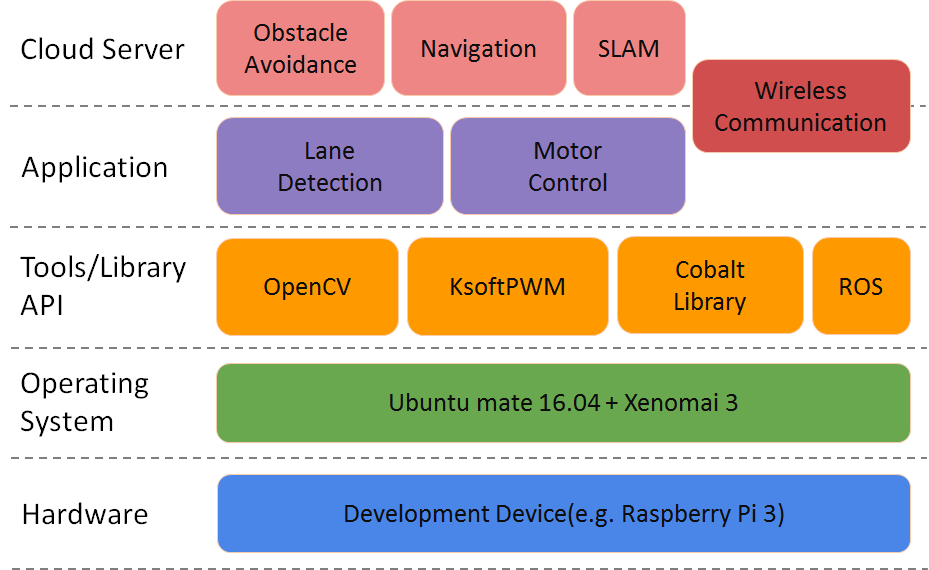
\includegraphics[width=3in]{img/arch.png}
	\caption{System Architecture}
	\label{fig:overall_arch}
\end{figure}

\subsection{Hardware}

Despite limited the budget shown in table \ref{hardware_list}, our autonomous vehicle prototype still has abilities of lane following, multiple car Interaction and route planning.

\begin{table}
	\centering
	\caption{Bill Of Materials}
	\label{hardware_list}
	\begin{tabular}{ll}
		Hardware                & Budgets  \\
		Raspberry Pi3 Model B   & 1200 NTD \\
		Raspberry Pi camera     & 698 NTD  \\
		2S LiPo battery 1300mAh & 240 NTD  \\
		Sandisk 16G microSD     & 185 NTD  \\
		L298N motor driver      & 263 NTD  \\
		Car frame               & 375 NTD  \\
		DC voltage regulator    & 105 NTD  \\
		Total                   & 3066 NTD
	\end{tabular}
\end{table}

\section{Implementation}

\subsection{Hard Real-Time Operating System}

RTOS guarantees the response time of real time task within specified time constraints \cite{RTOS}, often referred to as "deadline", and a hard real-time OS can always meet a deadline deterministically. We adopt Xenomai \cite{Xenomai}, an open source real-time Linux extension, allowing periodic preemptive hard real-time tasks along with typical Linux kernel and userspace. The Cobalt core in Xenomai 3 is a co-kernel which supplements the Linux kernel for delivering real-time services with very low latency \cite{rtlws2015}, shown in Figure \ref{fig:xeno_arch}, dealing with all time-critical events, such as interrupt handling, and scheduling real-time threads. Cobalt core, thereby has higher priority over Linux kernel. Our self-driving car benefits from deterministic behavior in Xenomai 3.

\begin{figure}
	\centering
	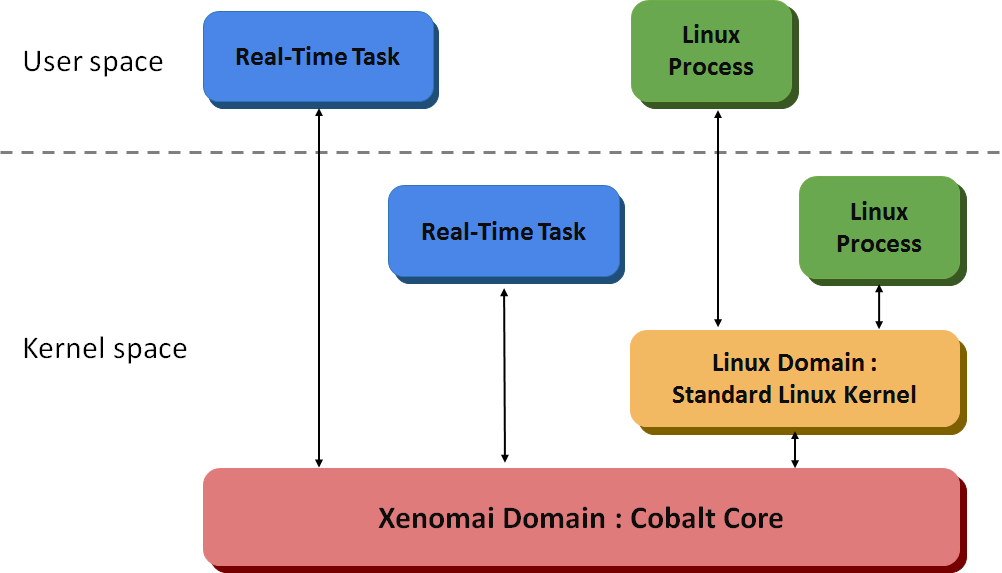
\includegraphics[width=3in]{img/xeno_arch.png}
	\caption{Cobalt core in Xenomai 3}
	\label{fig:xeno_arch}
\end{figure}

Most system use pulse width modulation (PWM) to simulate the analog signal for smooth motor controlling. PWM signals are often generated by certain hardware. On the contrary, using general-purpose input/output (GPIO) to simulate PWM signals is known as software PWM. We implement the later as a Xenomai kernel-mode real-time task to ensure the precision of PWM signal generation, named after KsoftPWM, for closed-loop control system, benefiting from the limination of system call overhead and potential locks.

\subsection{Lane Following Algorithm}

\subsubsection{Calibration}

Camera calibration is an early stage mission before performing computer vision operations. There are two sets of parameters needed to be found: intrinsic parameters and extrinsic parameter. By estimating them we can know the relation between 2D image plane and 3D world.

The intrinsic matrix describes the projection from 3D world into 2D image plane. The ideal linear model consists of focal length, pixel size and principal point. The nonlinear effect like lens distortion are also important, but it can not be described in the linear camera model, usually solved by numerical methods. Figure \ref{fig:intrinsic} shows the effect of intrinsic calibration; The extrinsic matrix describes the translation and rotation of camera with respect to the world frame, which means the angle and position of camera taking pictures in 3D world. Applying extrinsic matrix causes ground projection, showed in Figure \ref{fig:extrinsic}, which is like a bird eye view.

\begin{figure}
	\centering
	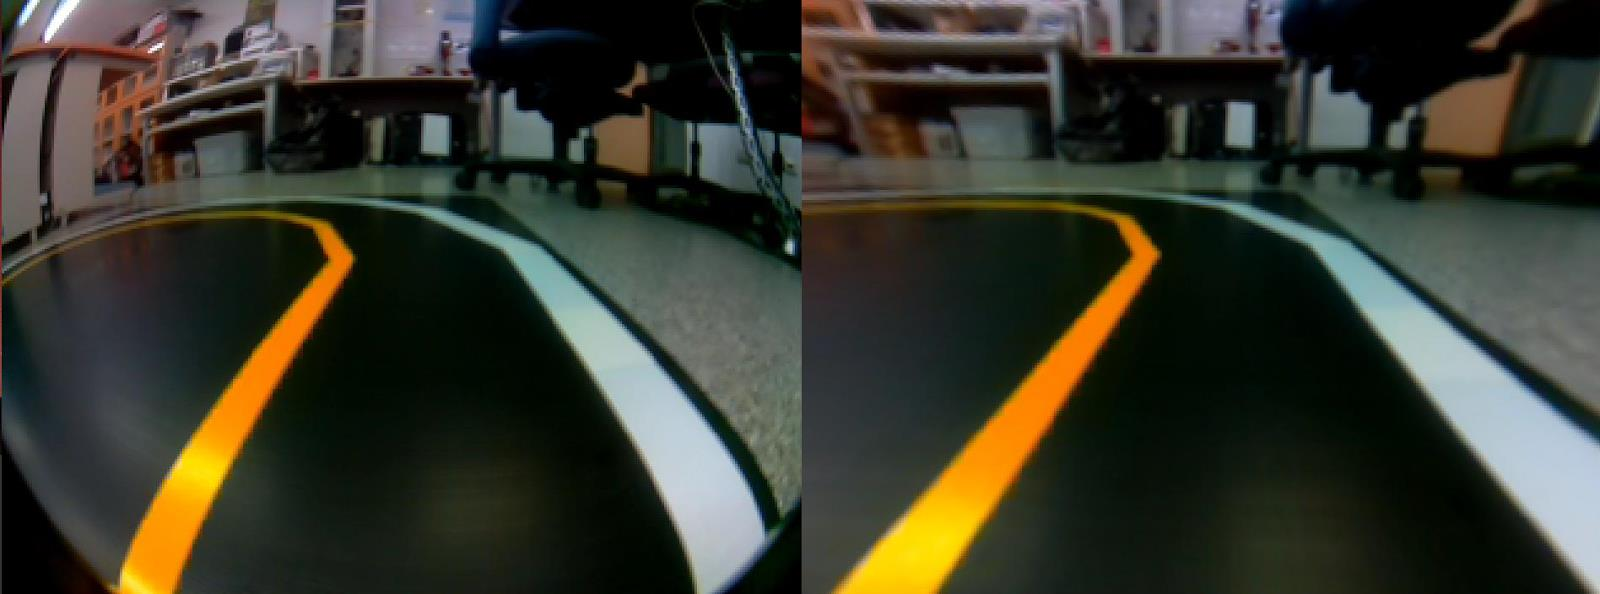
\includegraphics[width=3.5in]{img/intrinsic.png}
	\caption{Camera Undistortion}
	\label{fig:intrinsic}
\end{figure}

\begin{figure}	
	\centering
	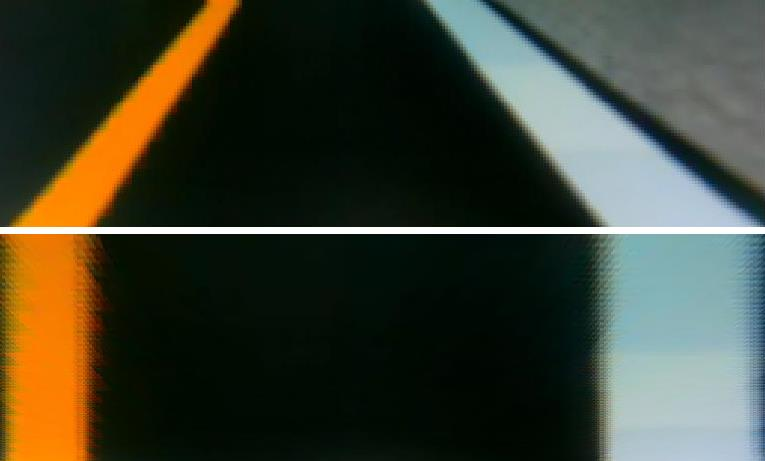
\includegraphics[width=2in]{img/extrinsic.png}
	\caption{Ground Projection}
	\label{fig:extrinsic}
\end{figure}

\subsubsection{Segment Detection}

Before pose estimation, we have to detect lane segments from the retrieved images in advance. It can be achieved by using Canny edge detection, color thresholding method and Hough transform. First, we transform the image from RGB color space into the HSV color space then use the color thresholding method to find the interested color like yellow or white in the image. Next, we apply Canny edge detection to detect the edges in the image, and use the bitwise and operation on color thresholding image and Canny edge image. This is a preparation step for Hough transform. Finally, apply the Hough Line transform comes out the segments.
 
Although the lane detector can find the segments, we still need to be aware of the side of lane mark that the segments is on, which is much important to pose estimation. Segment side can be determined by reading multiple pixels in both positive and negative direction of the segment normal vector on color thresholded image. Figure \ref{fig:lane_detect} visualizes the segment locations and segment sides, and also shows the values of $d$ and $\phi$. The lane detector only works at the bottom ROI(Region of Interest) part because there is much possible to be the lane.

\begin{figure}
	\centering
	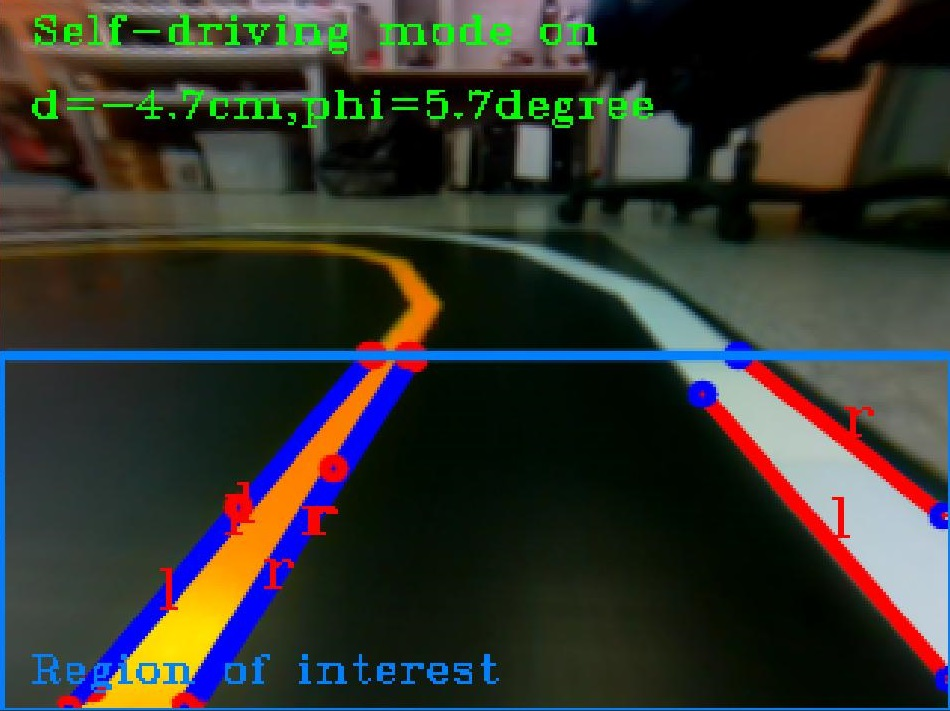
\includegraphics[width=2in]{img/lane_detect.png}
	\caption{Segments visualization}
	\label{fig:lane_detect}
\end{figure}

\subsubsection{Frame Transformation}

To reduce computation efforts, we apply extrinsic matrix that transforms the image from car's view to the road upper view to the segments, causing a straightforward coordinate parallel to lane. Moreover, the car camera is mounted in a distance from the origin. In order to know the real lateral displacement of the car, a transformation is needed for converting camera frame into car frame.

\subsubsection{Pose Estimation for Single Segment}

Due to the lane geometry, each of the segment that lane detector detects can be calculated to be a single pose data with respect to the lane, $d$ is the lateral displacement and $\phi$ is the orientation angle. We will put the data into the histogram filter for data filtering later. The process is similar to vote so we call it a vote generating function.

\subsubsection{Histogram Filter}

The segment poses generated in previous process will then be voted into the histogram filter. The histogram filter will find out the mode of these datas and eliminate the data out of the mode with certain range, i.e., the noise. After that, calculate the \textbf{mean} of the rest of the datas comes out a much accurate pose information.

\subsubsection{Controller}We build a differential wheeled car, on which there are two independent motors. The car can be turn by changing the speed rate between two motors, hence it does not require any additional steering mechanics. We use the well known algorithm \textbf{"PID controller"} to fix the orientation and lateral displacement.

The equation of PID controller in continuous time is given as:

\[e(t) = setpoint(t) - x(t)\]

\[u(t) = K_p e(t) + K_i \int_{0}^{t} e(\tau) d\tau + K_d  \frac{de(t)}{dt}\]

and for discrete time:

\[e[t] = setpoint[t] - x[t]\]

\[u[t] = K_p e[t] + K_i \sum_0^t e[t] \Delta t + K_d \frac{e[t] - e[t-1]}{\Delta t}\]

The pose controller is a cascaded PID controller. The $\phi$ controller is a low level controller for lane orientation stabilizing, and d controller fix the lateral displacement by changing the setpoint of $\phi$ controller to turn left or right.
The wheel control signal generating PWM is simply the throttle value plus the correction value:

\begin{lstlisting}
pwm_left = THROTTLE__BASE - pwm_correction
pwm_right = THROTTLE__BASE + pwm_correction
\end{lstlisting}

\begin{figure}	
	\centering
	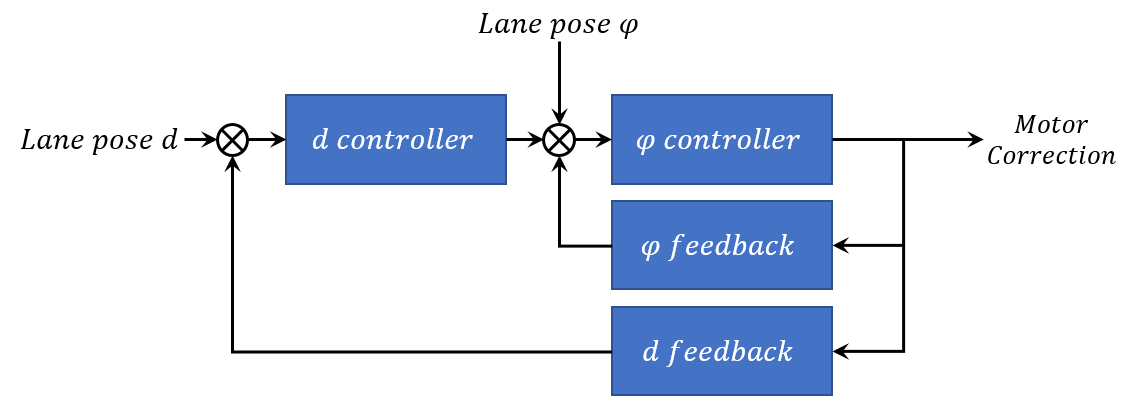
\includegraphics[width=3.5in]{img/controller.png}
	\caption{Control Diagram}
	\label{fig:controller}
\end{figure}

\subsection{Multiple Car Interaction}

\subsubsection{Apriltag}

Apriltag is a visual fiducial system. It appears as 2D bar code and stores data like QRcode. The difference is that Apriltag contains less data but provides farther and clearer data fetching, regardless of the orientation of view. Thus, it is useful for a wide variety of tasks including augmented reality, robotics, and camera calibration. The AprilTag detection software computes the precise 3D position, orientation, and identity of the tags relative to the camera. The 36h11 Apriltag family is adopted in this project to simulate scenario, like intersections, bus stops, traffic signal and parking lot.

\subsubsection{Crossroad}

Instead of using traditional and inefficient traffic light, we implement central management toward city crossroads. Before crossing a intersection, cars send request to the server according to the apriltag nearby which determines the crossroad ID. We predefine several states when multiple car intend to pass through the crossroad. For some situation, cars can pass at the same time, and others cannot, whereas need to set a lock until one car leaves the crossroad.

\section{Performance}

We executed tasks in user space, kernel space and irq task respectively, to evaluate real-time capability. We also compare performance among KsoftPWM, non-real-time PWM kernel module (nRTPKM) and WiringPi \cite{WiringPi}, the most famous library for GPIO controlling on Raspberry Pi 3 (Broadcom bcm2709 SoC, 1.2GHz ARM Cortex-A53 CPU). The background system load was generated by Linux Test Project (LTP), which provides a collection of tools for validating the reliability, robustness, and stability of Linux. Unit of latency is microsecond in all measurement.

\begin{figure}	
	\centering
	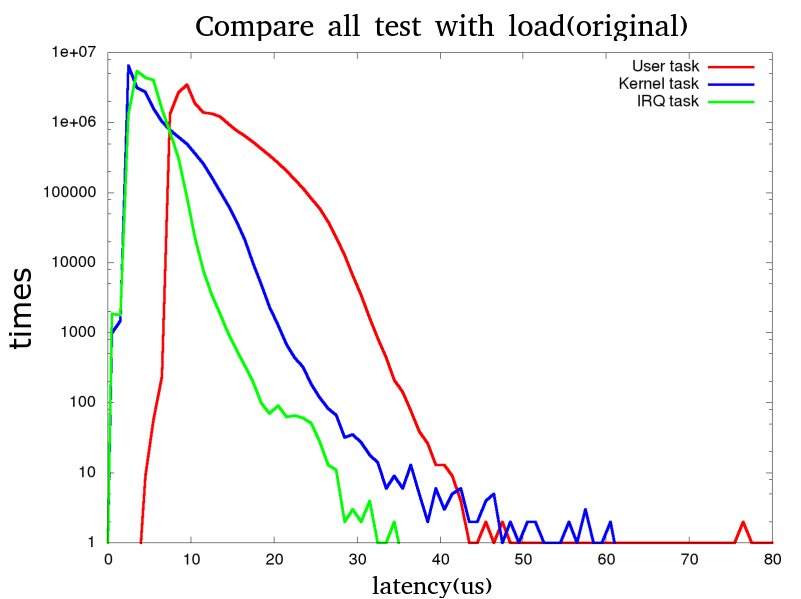
\includegraphics[width=2in]{img/xenomai_load.png}
	\caption{Xenomai Performance}
	\label{fig:xeno_perf}
\end{figure}

\begin{figure}
	\centering
	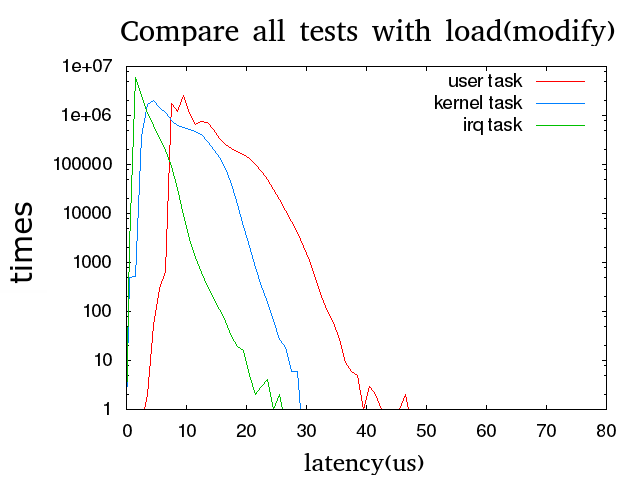
\includegraphics[width=2in]{img/xenomai_load_modify.png}
	\caption{Customized Xenomai Performance}
	\label{fig:xeno_perf_modify}
\end{figure}

\begin{table}[]
\centering
\caption{Maximum latency for Xenomai}
\label{xeno_compare}
\begin{tabular}{llll}
                              & User task & Kernel task & Irq task \\
Xenomai with original kernel  & 76.067 us & 36.262 us   & 27.895us \\
Xenomai with customized kernel & 42.678us  & 29.973us    & 27.11us 
\end{tabular}
\end{table}

\subsection{System Real-Time Performance}

Real-time performance is measured by stressing the system with LTP and applying cyclictest. We use LTP $-i$ and $-c$ flags to present the background CPU load with multiple processes and accessing on IO bus. Our customized Linux kernel brings better real-time ability in both user and kernel space, shown in Figure \ref{fig:xeno_perf_modify}. Table \ref{xeno_compare} records the maximum latency for Xenomai.

\subsection{KsoftPWM}

The KsoftPWM outperforms in better real-time ability, shown in Figure \ref{fig:ksoftpwm_perf}. The latency distribution of WiringPi is similar to nRTPKM, since both of them are just normal Linux userspace tasks rather than hard real-time one. The difference of minimum latency between WiringPi and nRTPKM was caused by different implementation. nRTPKM uses sleep function to simulate the PWM signals while WiringPi uses busy-waiting delay which may cause higher system load.

\begin{figure}
	\centering
	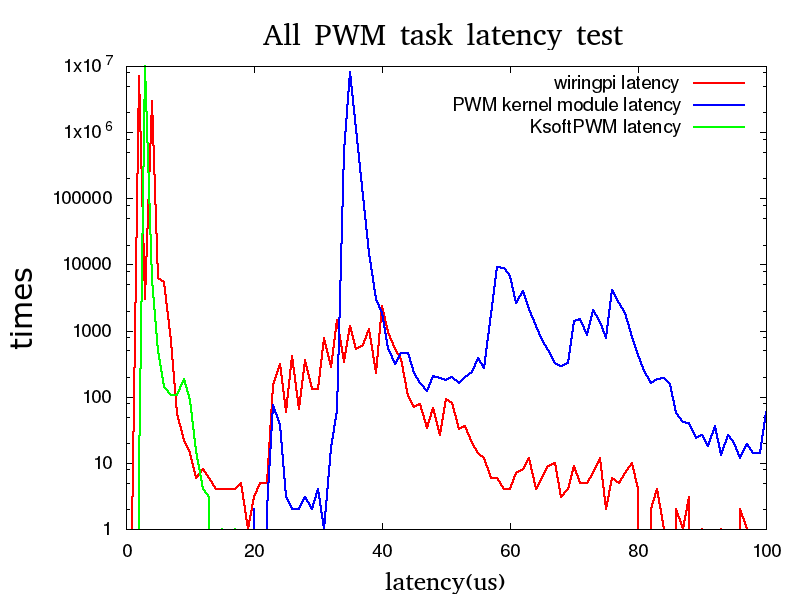
\includegraphics[width=2in]{img/ksoftpwm_load.png}
	\caption{PWM Task Performance}
	\label{fig:ksoftpwm_perf}
\end{figure}

\section{Conclusion}

This paper presents the hardware and software architecture of a self-driving miniature vehicle based entirely on cost-efficient components, that implies strategic values for the long term evaluation. RTOS should be very efficient in terms of resource usage and runtime. The context switching performance is important because the number of sensors can be high and we need to read data from different sensors continuously in real-time. Linux with real-time extension  fulfills all these criteria e.g., performance, reusability, changeability, and maintainability, whichhave significant value from the software engineer's perspective. Puyuma is released as an open source project as well as ROS, allowing further collaboration on algorithms and system integration.

\bibliographystyle{IEEEtran}
\bibliography{references}

\end{document}
